\documentclass[11pt,a4paper]{article}
\usepackage[margin=1in]{geometry}
\usepackage{amsmath,amssymb}
\usepackage{graphicx}
\usepackage{enumitem}
\usepackage{tcolorbox}
\usepackage{array}
\usepackage{multirow}
\usepackage{tikz}
\usepackage{xcolor}
\usetikzlibrary{positioning,arrows.meta,shapes}

% Custom commands
\newcommand{\highlight}[1]{\textbf{#1}}
\newcommand{\answer}[1]{\textcolor{blue}{\textit{#1}}}

% Box for exercises
\newtcolorbox{exercise}[1][]{
    colback=blue!5!white,
    colframe=blue!75!black,
    title=#1,
    fonttitle=\bfseries
}

\newtcolorbox{hint}[1][]{
    colback=yellow!10!white,
    colframe=orange!75!black,
    title=Hint,
    fonttitle=\bfseries
}

\newtcolorbox{concept}[1][]{
    colback=green!5!white,
    colframe=green!75!black,
    title=#1,
    fonttitle=\bfseries
}

\title{\textbf{Week 2: Word2Vec Deep Dive}\\
\large Understanding CBOW, Skip-gram, and Negative Sampling\\
\large Pre-Lab Exercise (No Programming Required)\\
\textcolor{red}{\textbf{INSTRUCTOR VERSION WITH ANSWER KEY}}}
\author{NLP Course 2025}
\date{}

\begin{document}
\maketitle

\noindent\textbf{Time:} 30-40 minutes\\
\textbf{Objective:} Master the core mechanisms of Word2Vec by understanding what goes in (context), how it's processed (method), and what comes out (prediction).

\section*{Part 1: Understanding Context Windows (10 minutes)}

\begin{exercise}[Context Window Discovery]
Consider this sentence: \textbf{``The quick brown fox jumps over the lazy dog''}

With a context window size of 2 (two words on each side), let's analyze the word ``fox'':

\textbf{Questions:}
\begin{enumerate}
    \item Circle the context words for ``fox'' (window size = 2):
    
    \texttt{The \quad \answer{quick} \quad \answer{brown} \quad \fbox{fox} \quad \answer{jumps} \quad \answer{over} \quad the \quad lazy \quad dog}
    
    \item What are the context words? \answer{quick, brown, jumps, over}
    
    \item For the word ``jumps'', what would be the context words (window size = 2)?
    
    Context words: \answer{brown, fox, over, the}
    
    \item \textbf{Key Question:} In a context window approach:
    \begin{itemize}
        \item What is the \textbf{CONTEXT}? \answer{The surrounding words within the window}
        \item What is the \textbf{METHOD}? \answer{Sliding window across the text}
        \item What is the \textbf{PREDICTION}? \answer{Word relationships based on co-occurrence}
    \end{itemize}
\end{enumerate}
\end{exercise}

\section*{Part 2: CBOW - Continuous Bag of Words (10 minutes)}

\begin{concept}[CBOW Principle]
CBOW predicts a target word given its surrounding context words. Think of it as a ``fill in the blank'' task.
\end{concept}

\begin{exercise}[CBOW in Action]
Given the sentence: ``The cat sat on the \underline{\hspace{1cm}} mat''

\textbf{Task 1: Manual CBOW}
\begin{enumerate}
    \item Context words given: [``cat'', ``sat'', ``on'', ``the'', ``mat'']
    
    What word would you predict for the blank? \answer{floor, ground, soft, old}
    
    \item Now consider: ``I love to \underline{\hspace{1cm}} pizza for dinner''
    
    Context words: [``I'', ``love'', ``to'', ``pizza'']
    
    Your prediction: \answer{eat, have, order}
\end{enumerate}

\textbf{Task 2: CBOW Analysis}
Complete the following table for CBOW:

\begin{center}
\begin{tabular}{|l|p{8cm}|}
\hline
\textbf{Aspect} & \textbf{Your Answer} \\
\hline\hline
INPUT (Context) & \answer{Multiple context words (surrounding words)} \\
& \\
\hline
METHOD & \answer{Average or sum the context word vectors,} \\
(How does it work?) & \answer{then predict the center word} \\
& \\
\hline
OUTPUT/PREDICTION & \answer{Single center/target word} \\
& \\
\hline
\end{tabular}
\end{center}

\textbf{Visual Representation:} Draw arrows showing the flow:
\begin{center}
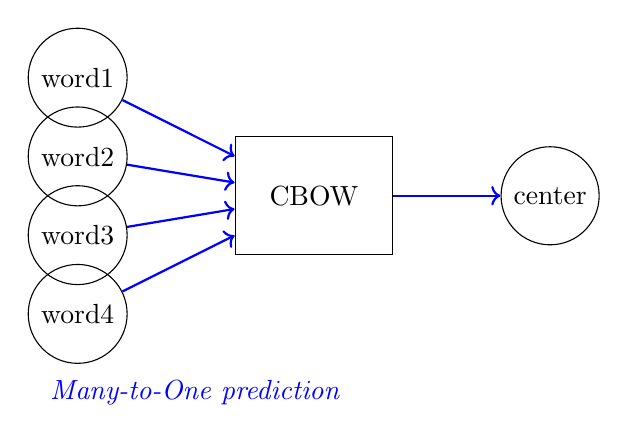
\begin{tikzpicture}
    % Input context words
    \node[draw, circle] (w1) at (0,2) {word1};
    \node[draw, circle] (w2) at (0,1) {word2};
    \node[draw, circle] (w3) at (0,0) {word3};
    \node[draw, circle] (w4) at (0,-1) {word4};
    
    % Model
    \node[draw, rectangle, minimum width=2cm, minimum height=1.5cm] (model) at (3,0.5) {CBOW};
    
    % Output
    \node[draw, circle] (out) at (6,0.5) {center};
    
    % Arrows - ANSWER
    \draw[->, thick, blue] (w1) -- (model);
    \draw[->, thick, blue] (w2) -- (model);
    \draw[->, thick, blue] (w3) -- (model);
    \draw[->, thick, blue] (w4) -- (model);
    \draw[->, thick, blue] (model) -- (out);
    
    \node[blue] at (1.5,-2) {\answer{Many-to-One prediction}};
\end{tikzpicture}
\end{center}
\end{exercise}

\section*{Part 3: Skip-gram - Predicting Context (10 minutes)}

\begin{concept}[Skip-gram Principle]
Skip-gram does the opposite of CBOW: given a center word, predict the surrounding context words.
\end{concept}

\begin{exercise}[Skip-gram in Action]
Given the center word ``\textbf{coffee}'' in: ``I drink coffee every morning''

\textbf{Task 1: Manual Skip-gram}
\begin{enumerate}
    \item What context words would you expect around ``coffee''? List 4 likely words:
    \begin{itemize}
        \item \answer{drink}
        \item \answer{morning}
        \item \answer{cup}
        \item \answer{hot}
    \end{itemize}
    
    \item Given center word ``\textbf{king}'', what context words might appear?
    \begin{itemize}
        \item \answer{queen, throne, crown, royal, palace}
        \item \answer{england, arthur, kingdom}
    \end{itemize}
\end{enumerate}

\textbf{Task 2: Skip-gram Analysis}
Complete the following table for Skip-gram:

\begin{center}
\begin{tabular}{|l|p{8cm}|}
\hline
\textbf{Aspect} & \textbf{Your Answer} \\
\hline\hline
INPUT (Context) & \answer{Single center/target word} \\
& \\
\hline
METHOD & \answer{Use center word vector to predict} \\
(How does it work?) & \answer{each context word independently} \\
& \\
\hline
OUTPUT/PREDICTION & \answer{Multiple context words (one at a time)} \\
& \\
\hline
\end{tabular}
\end{center}

\textbf{Task 3: CBOW vs Skip-gram}
\begin{enumerate}
    \item Which approach has MORE training examples from the same sentence?
    
    \answer{Skip-gram}
    
    \item Why? \answer{Skip-gram creates multiple training pairs (center, context1), (center, context2), etc., while CBOW creates one pair (all-context, center)}
\end{enumerate}
\end{exercise}

\section*{Part 4: Negative Sampling - Making Training Efficient (10 minutes)}

\begin{concept}[Why Negative Sampling?]
Training Word2Vec on large vocabularies (e.g., 50,000 words) is computationally expensive. Negative sampling speeds this up by only updating a small subset of weights.
\end{concept}

\begin{exercise}[Understanding Negative Sampling]
\textbf{Task 1: Positive vs Negative Pairs}

Given the sentence: ``The dog barked loudly''

With center word ``dog'' and context word ``barked'':
\begin{enumerate}
    \item This is a \answer{positive} pair because \answer{they actually appear together in context}
    
    \item Now consider ``dog'' and ``elephant''. This is a \answer{negative} pair because \answer{they don't appear together in this context}
    
    \item Create 3 negative pairs for center word ``dog'':
    \begin{itemize}
        \item (dog, \answer{computer})
        \item (dog, \answer{galaxy})
        \item (dog, \answer{mathematics})
    \end{itemize}
\end{enumerate}

\textbf{Task 2: The Sampling Process}

Instead of updating all 50,000 word weights, negative sampling:
\begin{enumerate}
    \item Updates the positive pair: (dog, barked) → predict ``1'' (real pair)
    \item Randomly samples k negative words (e.g., k=5)
    \item Updates these negative pairs: (dog, random\_word) → predict ``0'' (fake pair)
\end{enumerate}

\textbf{Complete this table for Negative Sampling:}

\begin{center}
\begin{tabular}{|l|p{8cm}|}
\hline
\textbf{Aspect} & \textbf{Your Answer} \\
\hline\hline
INPUT (Context) & \answer{Word pairs: 1 positive (real) pair} \\
& \answer{and k negative (random) pairs} \\
\hline
METHOD & \answer{Binary classification: predict 1 for positive pairs,} \\
(How does it work?) & \answer{0 for negative pairs. Update only k+1 weights} \\
& \\
\hline
OUTPUT/PREDICTION & \answer{Probability that a pair is real (0 or 1)} \\
& \\
\hline
\end{tabular}
\end{center}

\textbf{Task 3: Efficiency Analysis}
\begin{enumerate}
    \item Without negative sampling, how many weights update for each training example?
    
    \answer{All vocabulary weights (e.g., 50,000)}
    
    \item With negative sampling (k=5), how many weights update?
    
    \answer{Only 6 weights (1 positive + 5 negative)}
    
    \item What is the speedup factor for a 50,000-word vocabulary?
    
    \answer{50,000 / 6 ≈ 8,333x faster}
\end{enumerate}
\end{exercise}

\begin{hint}
Negative sampling converts the problem from multi-class classification (50,000 classes) to binary classification (real vs fake pairs).
\end{hint}

\section*{Part 5: Putting It All Together (5 minutes)}

\begin{exercise}[Synthesis]
Complete this comparison table:

\begin{center}
\begin{tabular}{|l|c|c|c|}
\hline
\textbf{Aspect} & \textbf{CBOW} & \textbf{Skip-gram} & \textbf{Negative Sampling} \\
\hline\hline
\textbf{Input} & Context words & \answer{Center word} & \answer{Word pairs} \\
& & & \\
\hline
\textbf{Method} & Average/combine & \answer{Predict each} & Binary \\
& context & \answer{context word} & classification \\
\hline
\textbf{Output} & \answer{Center word} & Context words & \answer{Real/fake (0/1)} \\
& & & \\
\hline
\textbf{Best for} & Frequent & \answer{Rare words} & \answer{Efficiency} \\
& words & & \\
\hline
\textbf{Training} & Faster & \answer{Slower but} & Makes both \\
\textbf{Speed} & & \answer{better quality} & faster \\
\hline
\end{tabular}
\end{center}

\textbf{Reflection Questions:}
\begin{enumerate}
    \item Why might Skip-gram work better for rare words than CBOW?
    
    \answer{Skip-gram generates more training examples per word occurrence. For a rare word appearing once with 4 context words, Skip-gram creates 4 training pairs while CBOW creates just 1. This gives Skip-gram more opportunities to learn about rare words.}
    
    \item How does negative sampling change what the model is learning to predict?
    
    \answer{Without negative sampling: predict which specific word (out of 50,000) comes next.}
    \answer{With negative sampling: predict whether a word pair is real (1) or fake (0) - binary classification instead of 50,000-way classification.}
    
    \item If you wanted to find similar words to ``doctor'', which approach (CBOW or Skip-gram) would likely give better results? Why?
    
    \answer{Skip-gram would likely give better results because it directly learns what context words appear around ``doctor'', capturing more nuanced relationships. CBOW averages context, potentially losing fine-grained distinctions that make ``doctor'' unique from related words like ``nurse'' or ``physician''.}
\end{enumerate}
\end{exercise}

\section*{Instructor Notes}

\subsection*{Key Teaching Points}

\begin{enumerate}
    \item \textbf{Context-Method-Output Framework}: Consistently emphasize this trilogy:
    \begin{itemize}
        \item CBOW: Multiple context → Average → Single word
        \item Skip-gram: Single word → Separate predictions → Multiple context
        \item Negative Sampling: Word pairs → Binary classification → Real/fake
    \end{itemize}
    
    \item \textbf{Intuitive Understanding}:
    \begin{itemize}
        \item CBOW = Fill in the blank (convergent thinking)
        \item Skip-gram = Word association (divergent thinking)
        \item Negative Sampling = Real or fake game
    \end{itemize}
    
    \item \textbf{Common Misconceptions}:
    \begin{itemize}
        \item Students often confuse input/output for CBOW vs Skip-gram
        \item Emphasize that negative sampling is an optimization technique, not a separate model
        \item Clarify that ``bag of words'' in CBOW means order doesn't matter
    \end{itemize}
    
    \item \textbf{Computational Insights}:
    \begin{itemize}
        \item Without negative sampling: O(V) operations per training example
        \item With negative sampling: O(k) operations, where k << V
        \item This makes training on billions of words feasible
    \end{itemize}
\end{enumerate}

\subsection*{Extension Questions}

For advanced students:
\begin{enumerate}
    \item How would you handle words that appear in multiple senses (e.g., ``bank'')?
    \item Why do we sample negative words based on frequency raised to 0.75 power?
    \item How does subsampling frequent words (like ``the'', ``a'') improve embeddings?
\end{enumerate}

\subsection*{Follow-up Programming Lab}

After this conceptual introduction, students will be ready to:
\begin{itemize}
    \item Implement a simple CBOW model in Python
    \item Visualize Skip-gram training pairs from real text
    \item Compare embeddings with and without negative sampling
    \item Explore pre-trained Word2Vec models
\end{itemize}

\vspace{1cm}
\noindent\rule{\textwidth}{0.4pt}
\begin{center}
\textit{End of Instructor Version}
\end{center}

\end{document}